\documentclass[conference]{IEEEtran}
\IEEEoverridecommandlockouts
% The preceding line is only needed to identify funding in the first footnote. If that is unneeded, please comment it out.
\usepackage{cite}
\usepackage{amsmath,amssymb,amsfonts}
\usepackage{algorithmic}
\usepackage{graphicx}
\usepackage{textcomp}
\usepackage{xcolor}
\usepackage{caption}
\usepackage{float}
\def\BibTeX{{\rm B\kern-.05em{\sc i\kern-.025em b}\kern-.08em
    T\kern-.1667em\lower.7ex\hbox{E}\kern-.125emX}}
\begin{document}

\title{Deep Learning for Plant Recognition}

\author{\IEEEauthorblockN{Olaniyi Bayonle Alao}
\IEEEauthorblockA{\textit{Electronic Engineering} \\
\textit{Hochschule Hamm-Lippstadt}\\
Lippstadt, Germany \\
olaniyi-bayonle.alao@stud.hshl.de}

}

\maketitle

\begin{abstract}
Plant recognition is an essential yet challenging task. Leaf recognition is a vital part of plant recognition, and a good extraction of the unique features in different leaves leads to a robust plant recognition system. Until recently, the combination of computer vision and machine learning techniques have been used for classifying plants. However, these techniques require a lot of manual processes for feature extraction. This paper presents Convolutional neural networks (CNN) architectures for automatic feature extraction and classification in plant recognition. Experimental results showed the effectiveness of CNN architectures, most especially ResNet-152, with an accuracy of 100\% for plant recognition tasks.

\end{abstract}

\begin{IEEEkeywords}
deep learning, plant recognition, CNN, AlexNet, ResNet
\end{IEEEkeywords}

\section{Introduction}
Identifying different species and types of plants growing in our natural habitat has long been an important task. However, these tasks have not been easy due to the abundance of plant species we have and the fact that many plants have a lot of similar characteristics. Therefore, experts in the field of agriculture have been trying to identify and document these plants correctly. However, experts also find the task of identifying plant species difficult due to their abundance and characteristics.

With many plants on the verge of going into extinction and biodiversity at risk \cite{pimm2015many}, there has been an increase in the need to reduce the task of experts in plant species conservations to be able to identify plants as easy and less time consuming as possible. From a farmer's point of view, it is crucial to have a system in place that can differentiate between desired plants and unwanted plants - weeds. The automatic detection and controlling of weeds with herbicides using robotics will allow for precise farming, which will, in turn, increase the yields from a planting season \cite{bah2018deep}. This exact treatment for plants with what they need can reduce farmers' investment, potentially leading to greater profits. In addition, the precise use of herbicides on detected weeds can contribute to a reduction in the environmental pollutions caused by the traditional way of spraying herbicides evenly across farmland.

Recently, researchers have trialled the use of machine learning algorithms to identify plant species through leaf images. The use of this technique is possible since expert botanists often use leaf shape, colour and textures amongst other things for plant leaf classification task \cite{xiao2010hog, kadir2013leaf}. However, using computer vision which is a subset of machine learning, for this task has proven to be challenging \cite{kamilaris2018deep}. These challenges are because the feature used for leaf identifications and classifications were hand-crafted into these algorithms. Hand-crafting these features meant that the algorithm did not learn to do the classification job independently. Hence it is prone to the same errors expert botanists will make.

Deep learning techniques have been explored and have shown tremendous results to solve these challenges with using computer vision for leaf image classification. The success of deep learning has been attributed to the advancement in the capabilities of graphics processing units (GPU), which can now perform computationally expensive deep learning tasks at incredible speeds \cite{campbell2020explosion}. The essential advantage of deep learning over the other traditional machine learning techniques is its ability to automatically extract critical features from the input data using the characteristics of its deep neural networks. Several research studies have shown that convolutional neural networks (CNN) are best suitable for image classification jobs out of the deep learning neural network types.

Zhu et al. \cite{zhu2019ta} proposed two-way attention models for further optimisation in discriminative feature learning and part based attention using deep CNN for automatic plant recognition. The results of their method trained with Xception architecture on four different datasets: Malayakew, ICL, Flowers 102 and CFH plant, produced accuracies of 99.8\%, 99.9\%, 97.2\% and 79.5\%, respectively.

Pawara et al. \cite{pawara2017comparing} compared models trained using local feature descriptors and bags of visual words with different classifiers to deep CNN models on three plant datasets; AgrilPlant, LeafSnap, and Folio. They trained their CNN models using scratch and fine-tuned GoggleNet and AlexNet architectures. Their other models trained using KNN, SVM, and MLP to classify their hand-crafted extracted features. Their studies found that their deep CNN methods outperformed the hand-craft extracted features.

Anubha et al. \cite{anubha2019study} conducted a study on using conventional image processing and deep learning techniques for plant recognition tasks. Their conventional image processing techniques include using classifiers like random forest and SVM on manually extracted features. For deep learning techniques, the features automatically extracted using CNN based architectures were categorised using classifiers like logistics regression. The study used Folio, Swedish leaf, and Flavia datasets to train their models. They observed that models trained and classified using CNN based architectures performed better than ones trained using conventional image processing techniques.

Thanks to the capabilities of CNN, a new dawn has been set in making the task of plant recognition relatively easy and robust for interested individuals. Deep learning models are currently helping millions of agricultural professionals and hobbyists in the correct plant species identification through mobile applications like Leafsnap and Pl@ntNet \cite{kumar2012leafsnap, plantnet_team}.

This paper compares the accuracies of pre-trained AlexNet and ResNet CNN architectures for plant recognition on the Agriplant and Swedish leaf plant datasets. The rest of the paper is structured as follows: Section 2 begins with a description of the theoretical background of CNN. The section continues with a brief overview of the CNN architectures used to train the plant recognition models, the datasets used, and the hardware and software used to train the models. Section 3 of the paper presents the results of the research. Finally, sections 4 and 5 discussed the research results and concluded the paper with propositions for further research.





\section{Materials and Methods}


\subsection{Deep Learning}\label{AA}

In the past, image classifications workflows consist of processes like image pre-processing, feature extractions and finally classification with machine learning algorithms like support vector machine (SVM), random forest (RF), K-nearest neighbour (KNN), amongst others. The shape, colour, texture and vein were among the features extracted from the leaf images using methods like local binary pattern and Gabor filter  \cite{guo2010completed, li2010selection}. Furthermore, shape and colour extraction techniques like scale space, discrete wavelet transform (DWT) and comparing the colour of images to predefined reference colours are used to extract these features \cite{satpute2016color}. However, the lack of automation of this process made them impractical for broad adoption. Currently, deep learning methods, particularly CNN, are used to classify plants using leaf images \cite{sardogan2018plant}.


Deep learning is a model to learning for computers that have some of its bases on the understanding of how the human brain learns complex and specific things \cite{wang2017origin}.
Out of the subset of machine learning, deep learning is the most active field \cite{angermueller2016deep}.

\subsection{Convolutional Neural Networks}
Convolutional neural networks are a type of neural network in DL designed for processing grid-like or multi-array kinds of data \cite{lecun2015deep,goodfellow2016deep}. These neural networks typically consist of an input image, convolution, pooling and fully connected layers. The networks architecture of CNN allows them to train on deep layered data structures at a fast pace and robust in the correct classification of images \cite{nielsen2015neural}. The achievement of these capabilities are possible through the use of four essential components - the use of many layers, local connections, shared weights, and pooling \cite{lecun2015deep}.

\subsubsection{Convolutional layer}
This layer performs mathematical operations on the input image to extract the so-called feature map by using a filter - kernel \cite{goodfellow2016deep}. The feature map is obtained by summing results gathered from the multiplication of pixel by pixel value and kernel values as the function scans the image from the top left corner down to the bottom right of the picture. This operation results in a smaller size version of the input image. Figure 2 shows a representation of this operation.

A padding operation of the original pixel matrix ensures that all pixels, mainly the corner pixels in the input image, participate in multiple convolution/feature detection operations. This is achieved by adding arbitrary numbers of pixels around the boundaries of the original image. For example, padding of two translates to adding two extra pixels around the borders of the original image matrix. The scanning of the image pixels is called stride, i.e. the number of pixels the filter moves over the input image pixels. For example, a stride value of 3 means that the filter moves by 3 pixels over the image.


\subsubsection{Pooling layer}
The pooling layer is the next layer after the convolution layer. The reduction of features extracted from convolutional operations performed in the preceding layer occurs in the pooling layer. For example, Max pooling operation chooses the maximum value within a rectangular quarter while average pooling takes the average of the values in each area \cite{goodfellow2016deep}.
Achieving non-linearity in the learned networks is made possible by an activation function.
An activation function is a function that ensures non-linearity in the networks by determining the activation of neurons in the convolutional and pooling layer \cite{nielsen2015neural}. Rectified Linear Unit (ReLU) is CNN's most commonly used activation function.



\subsubsection{Fully Connected Layer}
Recognition and classification of extracted data from previous layers occur in this layer. The neurons directly connect to all activated neurons in the pooling layers in this layer. The outputs in this layer result from the direct connection to all activated neurons in the max pooled layer. Figure \ref{fig:train_gate} shows an overview of the layers in a general CNN architecture.

This paper uses a pre-trained CNN architecture because characteristics learned in a pre-trained CNN model on large datasets can be fine-tuned for a new task \cite{zhuang2020comprehensive}. Likewise, there is insufficient diversity in the paper's dataset for training a CNN model from scratch. Hence the reason for resolving to a pre-trained CNN architecture - AlexNet and ResNet. 


    \begin{figure}[htbp]
        \centerline{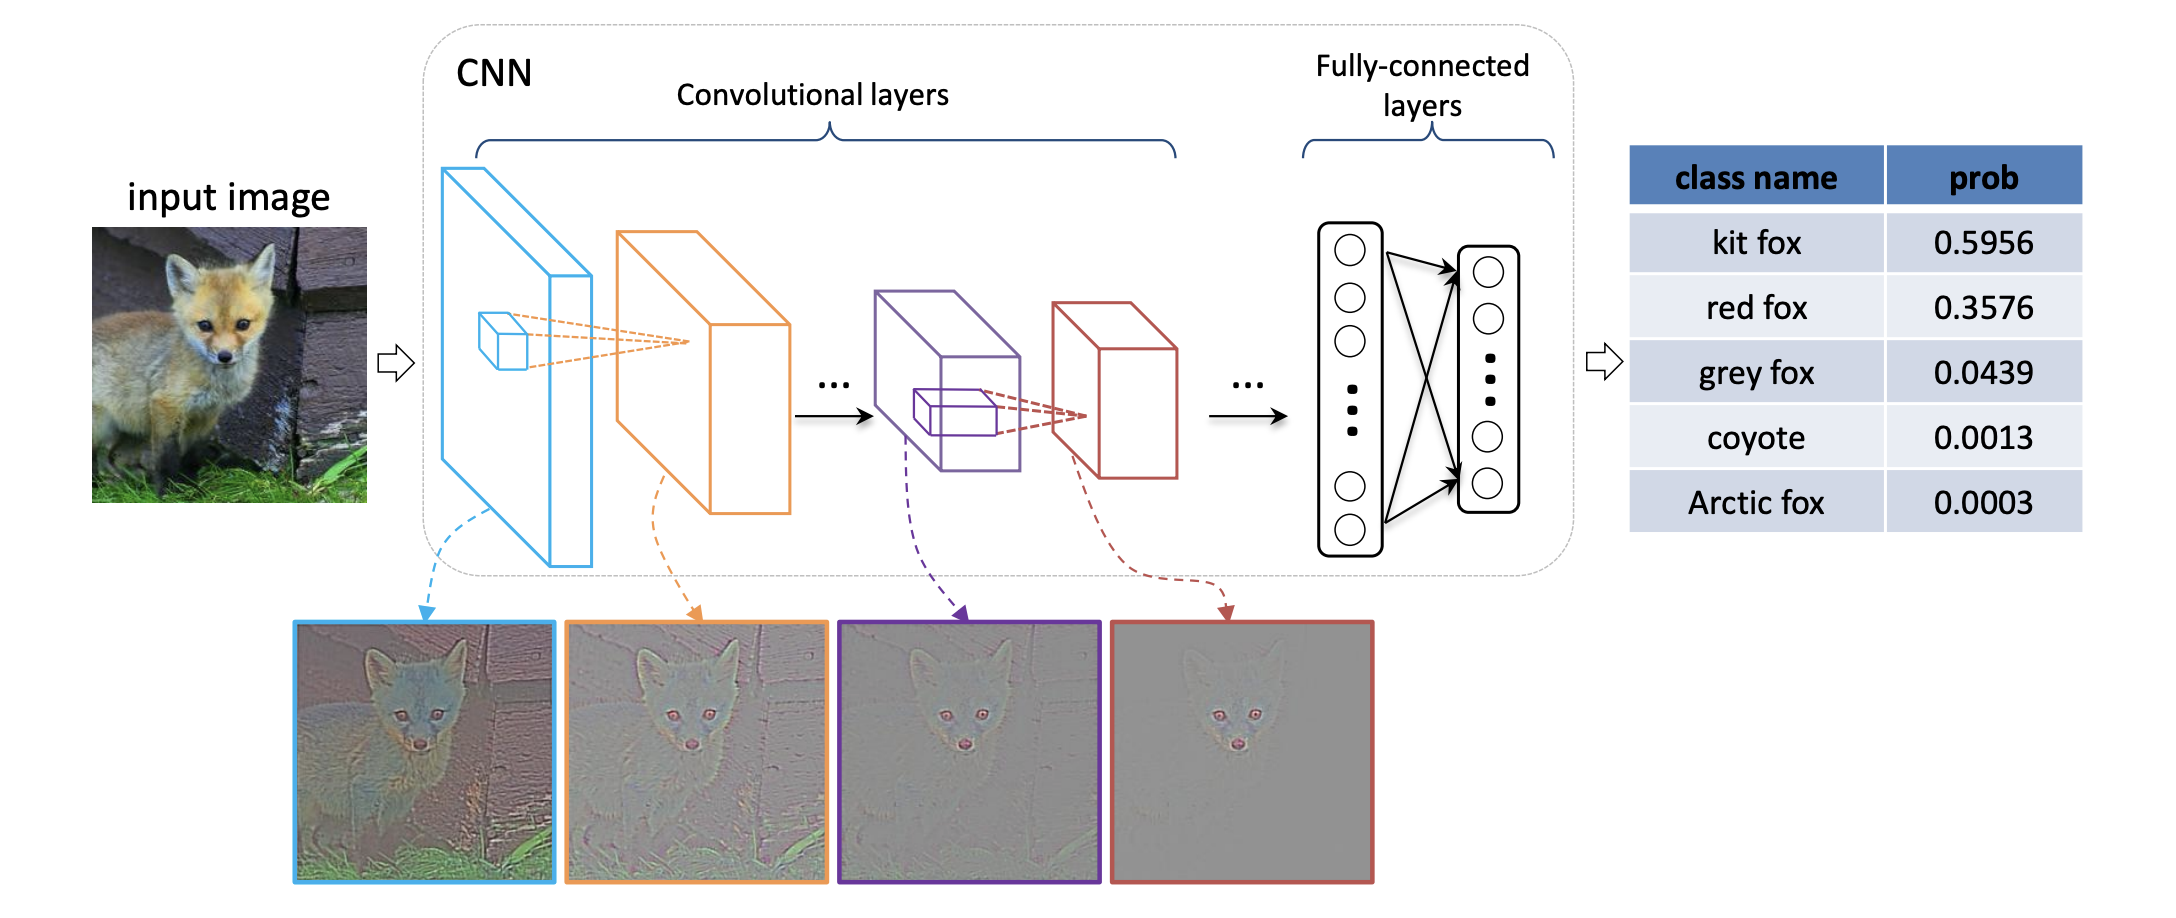
\includegraphics[scale=0.25]{figures/Screenshot 2021-11-24 at 14.35.12.png}}
        \caption{Screenshot showing an overview of the convolutional and full-connected layers in CNN architecture and the oupt of each layer on the input image \cite{soderkvist2001computer}}

        \label{fig:train_gate}
    \end{figure}
    

\subsection{CNN Architectures used (AlexNet, ResNet-34)}
The paper used the AlexNet and ResNet-34 architectures to train the experiment's model.

AlexNet is a CNN architecture introduced by \cite{krizhevsky2012imagenet}. AlexNet architecture consists of 8 weight layers: five convolutional layers and three fully connected layers. The first, second and fifth convolutional layers are each followed by normalisation and a max-pooling layer. The first convolutional layer filters the input image with 96 kernels of 11 x 11 in size and a stride of 4 pixels. The second layer filters the input of the first convolutional layer with 256 kernels of size 5 x 5 and a stride of 1 pixel. The third, fourth, and fifth convolutional layers have 384, 256 and 384 kernels with sizes 3 x 3. The fully connected layers have 4,096 neurons each, and the RELU non-linearity function is applied to the output and convolutional layers.
The pre-trained network of AlexNet on the ImageNet dataset can classify images into 1000 object categories.

Likewise, ResNet-34 is a CNN network architecture with 34 deeper weight layers introduced by \cite{he2016deep}. The ResNet architecture turns a plain neural network (VGG nets but with fewer filters and lower complexity) into a residual network by inserting shortcut connections between the original network layers. The shortcut connections fix the vanishing gradient problem in the deep CNN network by creating an alternative bypass for the gradient by adding outputs from previous layers to that of the stack layers. Figure \ref{fig:resnet} shows the network architecture of ResNet-34 in comparison with that of plain CNN. Both architectures figure \ref{fig:resnet} are 34 layers deep, but ResNet has a connection between all the layers.
There are different variants of the ResNet architecture. The number in each variant depicts the number of layers in the residual network. Examples are ResNet-18, ResNet-50, ResNet-101, ResNet-110, ResNet-152, ResNet-164, and ResNet-1202.


    \begin{figure}[ht!]
        \centerline{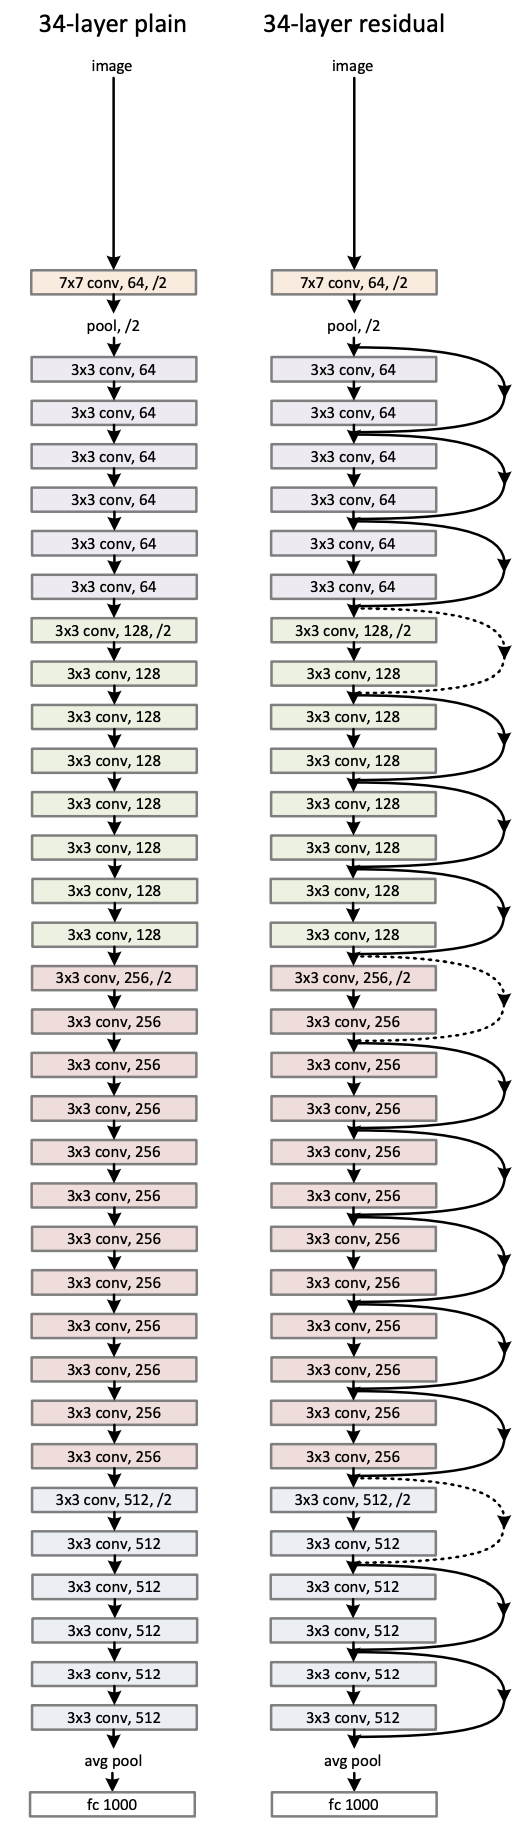
\includegraphics[scale=0.32]{figures/Screenshot 2021-12-16 at 17.28.47.png}}
        \caption{Screenshot showing an overview of ResNet-34 architecture in comparison with plain CNN architecture \cite{he2016deep}}

        \label{fig:resnet}
    \end{figure}
    



\subsection{Dataset}
The paper performed the experiments using 2 standard datasets; Swedish leaf \cite{soderkvist2001computer} and AgrilPlant \cite{pawara2017comparing}.

\subsubsection{Swedish Leaf Dataset}
For plant recognition researches, \cite{soderkvist2001computer} published the Swedish leaf dataset. This dataset consists of 1125 leaf images from 15 different plant species classes. Thus, each plant species contains precisely 75 images. The tree classes are Ulmus carpinifolia, Acer, Salix aurita, Quercus, Alnus incana, Betula pubescens, Salix alba 'Sericea', Populus tremula, Ulmus glabra, Sorbus aucuparia, Salix sinerea, Populus, Tilia, Sorbus intermedia, Fagus silvatica. The leaf images of each plant species were in a laboratory on a white background. Figure \ref{fig:gate4} shows sample images from the Swedish leaf dataset.


\subsubsection{AgrilPlant Dataset}
 \cite{pawara2017comparing} introduced the AgrilPlant dataset for plant recognition tasks. This dataset consists of precisely 300 images of 10 classes of plants, amounting to a total of 3000 images. Flickr website is the source of the images in this dataset. The images may contain the landscape of the entire plant, branch, leaf, fruit and flower. The Agrilplant dataset is very challenging because of the following reasons:
 
 \begin{itemize}
     \item There are similarities among some classes, i.e. apple, orange, and persimmon, which have similar shapes and colours.
     \item There is a diversity of plants within the same class. For example, there are green and red apples or varieties of tulips.
     \item The images contain various objects in the background not relevant to the recognition task. These background noises are from the outdoor environments where the images were taken.
     \item There is a similarity among some classes. For example, apple, orange, and persimmon images have similar shapes and colours.

Figure \ref{fig:agrilplant} shows sample images from the AgrilPlant dataset.

 \end{itemize}
 
%  \clearpage
    \begin{figure}
   

        
        \centerline{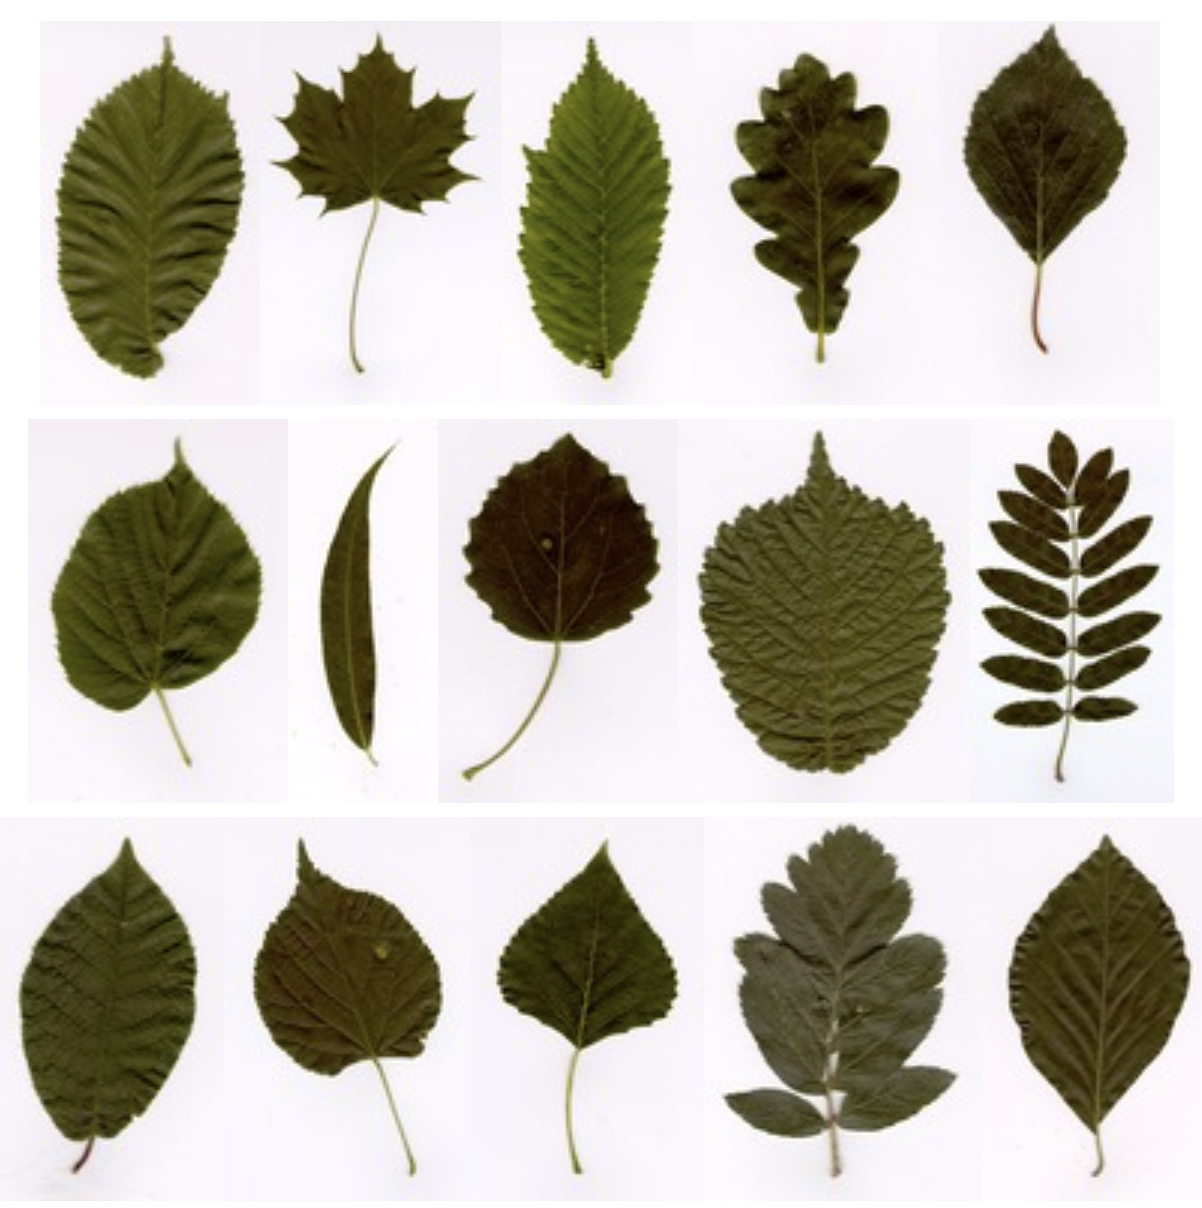
\includegraphics[scale=0.25]{figures/Screenshot 2021-11-25 at 13.34.07.png}}
         \caption{Screenshot showing sample images from the classes in the Swedish leaf dataset \cite{soderkvist2001computer}.}

        \label{fig:gate4}
    \end{figure}




    

\subsection{Hardware, Software and Parameter settings}
The paper used Jupyter Notebooks \cite{kluyver2016jupyter} running Python 3 kernels with the PyTorch \cite{paszke2017automatic} and fast.ai \cite{howard2018fastai} libraries for training and evaluating the CNN models on a Linux server with 32 GB of RAM and a GTX 1080 GPU with 8 GB of RAM.

In the experiment, all images in the dataset were rescaled to 256 x 256 pixels for better classification and part localisation. The paper used Adam \cite{kingma2014adam} for optimising the models, learning rate of 0.001, 80\% of the dataset for training and 20\% for testing. Each pre-trained CNN architecture was trained for five epochs on the dataset.

    \begin{figure*}
    
        \centerline{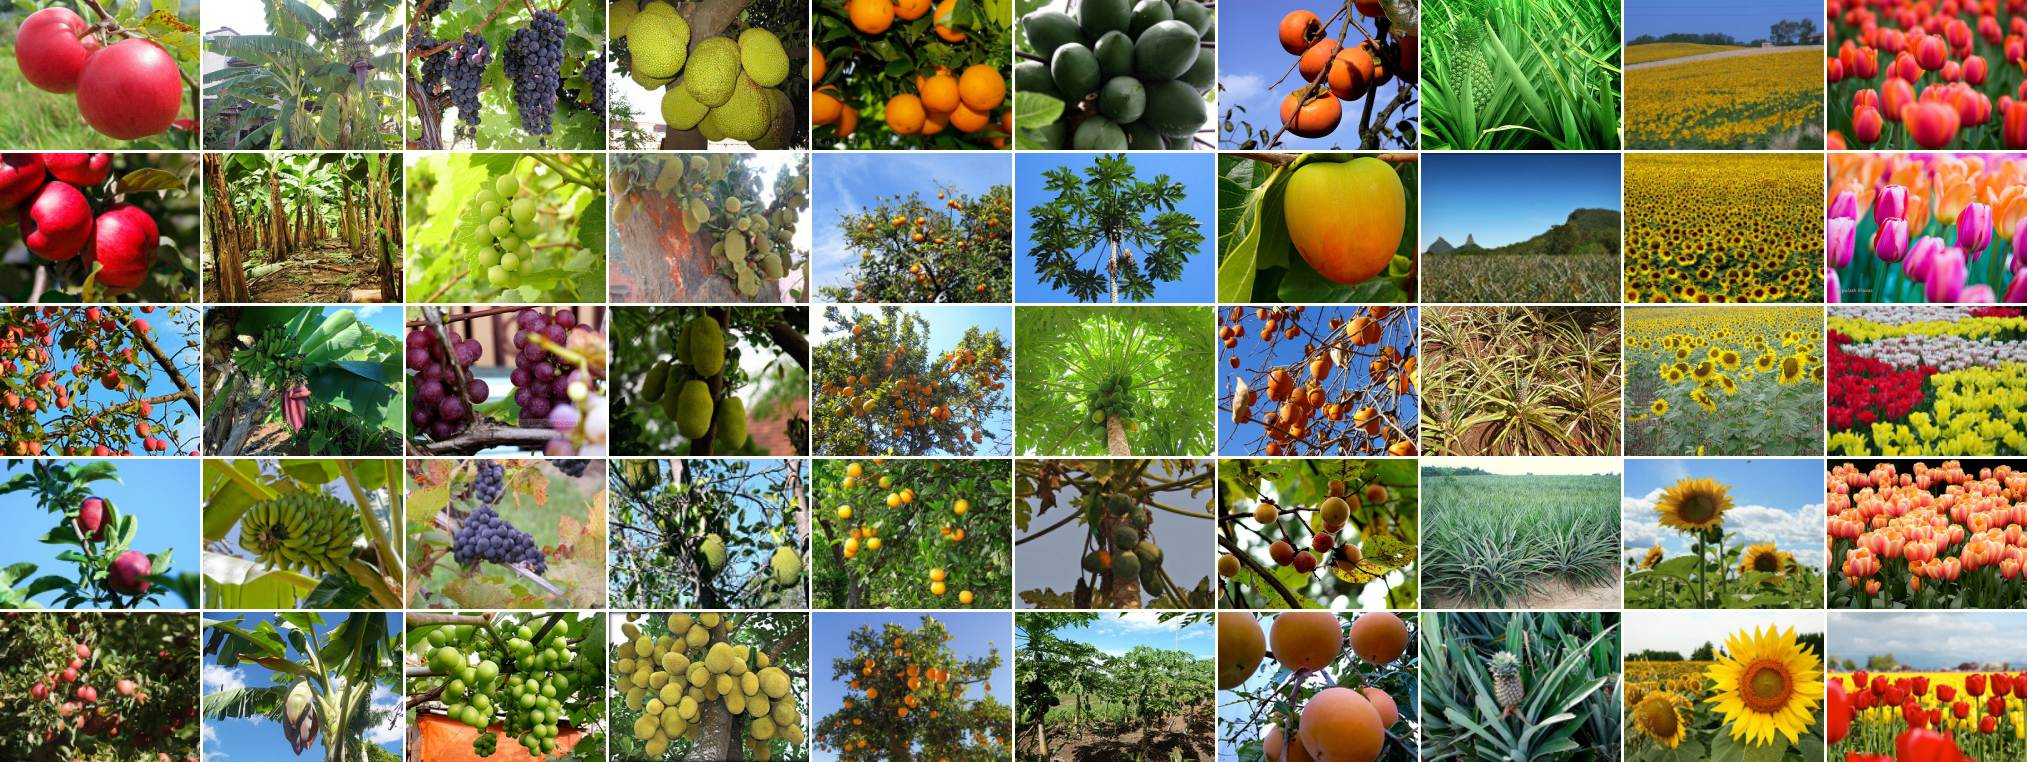
\includegraphics[width=1\textwidth]{figures/agrilplant-image.jpeg}}
        \caption{Screenshot showing sample images from the classes in the AgrilPlant dataset \cite{pawara2017comparing}}

        \label{fig:agrilplant}
    \end{figure*}
    
%     \noindent%
% \begin{minipage}{\linewidth}% to keep image and caption on one page
% \makebox[\linewidth]{%        to center the image
%   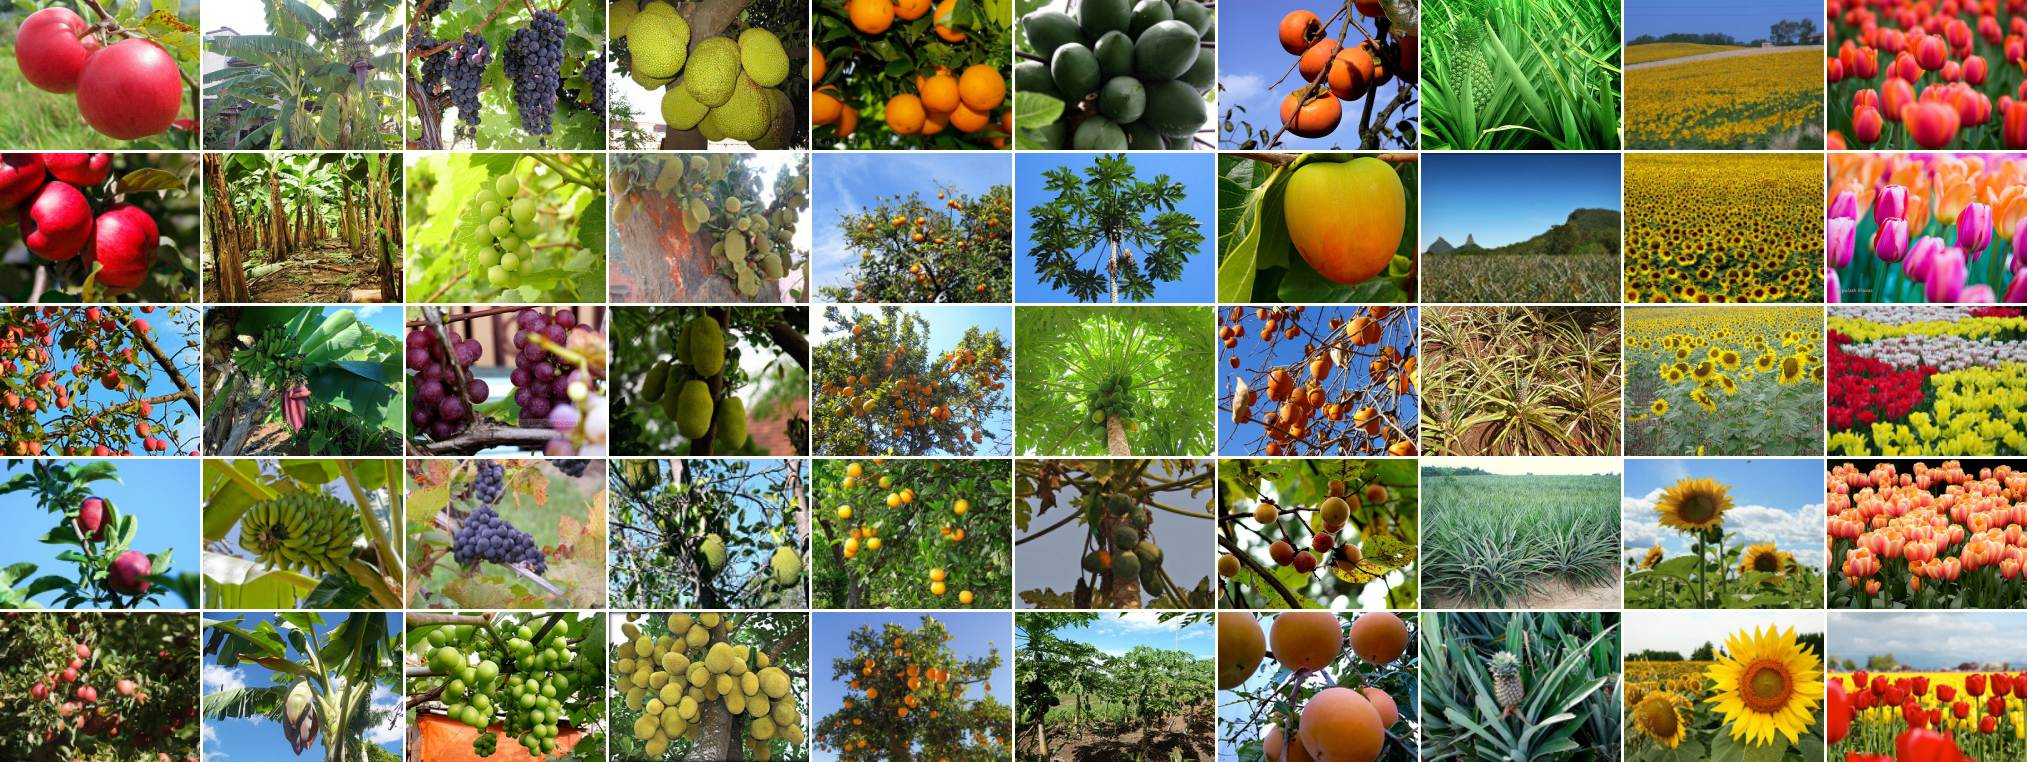
\includegraphics[keepaspectratio=true,scale=0.6]{figures/agrilplant-image.jpeg}}
% \captionof{figure}{...}\label{visina8}%      only if needed  
% \end{minipage}
        

\section{Results}
\subsubsection{Swedish Leaf Dataset Evaluation} 
Table \ref{tab1} shows the classification accuracy, training time, and total parameters in the trained CNN architectures on the Swedish leaf dataset. ResNet-50 and ResNet-152 achieved the best performance with an accuracy of 100\% in classifying the leaves in the Swedish leaf dataset. However, ResNet-50 had less training time and total parameters than ResNet-152 despite having the same accuracy. On the other hand, AlexNet performed the least in the classification task with an accuracy of 98.7\% using the least total parameters compared to other architectures. The AlexNet accuracy reported by Pawara et al. \cite{pawara2017data} outperforms the AlexNet accuracy in this study. The accuracy of the ResNet-50 and ResNet-152 models in this study exceeds that reported by Anubha et al. \cite{anubha2019study} using VGG-16 (98.52\%) and VGG-19 (99.41\%) architectures.
\begin{table}[htbp]
\caption{Comaparison of the classification accuracy, training time, and total parameters between CNN methods trained on the Swedish leaf dataset.}
\begin{center}
\begin{tabular}{c|c|c|c}

\textbf{Methods} & \textbf{Accuracy}& \textbf{Total Parameters}& \textbf{Training Time (s)} \\
\hline
\hline
ResNet-18 & 99.6\%& 11,711,552 & 05 \\
\hline
ResNet-34 & 99.1\%& 21,819,712 & 05 \\
\hline
ResNet-50 & 100\%& 25,622,080 & 08 \\
\hline
ResNet-101 & 99.6\%& 44,614,208 & 10 \\
\hline
ResNet-152 & 100\%& 60,257,856 & 14 \\
\hline
AlexNet & 98.7\%& 2,741,568 & 06 \\

\end{tabular}
\label{tab1}
\end{center}
\end{table}

\subsubsection{AgrilPlant Dataset}
For the AgrilPlant dataset, ResNet-152 obtained the best performance with a classification accuracy of 99.3\% and the highest average training time of 28 seconds per epoch. The ResNet-152 model accuracy outperforms the accuracy reported by Pawara et al. \cite{pawara2017comparing}. Table \ref{table:agril} shows the result of ResNet and AlexNet architectures of the datasets. 

\begin{table}[htbp]
\caption{Comaparison of the classification accuracy, training time, and total parameters between CNN methods trained on the AgrilPlant dataset.}
\begin{center}
\begin{tabular}{c|c|c|c}

\textbf{Methods} & \textbf{Accuracy}& \textbf{Total Parameters}& \textbf{Training Time (s)} \\
\hline
ResNet-18 & 98.2\%& 11,708,992 & 07 \\
\hline
ResNet-34 & 99.2\%& 21,817,152 & 07 \\
\hline
ResNet-50 & 99.2\%& 25,619,520 & 14 \\
\hline
ResNet-101 & 99\%& 44,611,648 & 20 \\
\hline
ResNet-152 & 99.3\%& 60,255,296 & 28 \\
\hline
AlexNet & 96.3\%& 2,739,008 & 04 \\

\end{tabular}
\label{table:agril}
\end{center}
\end{table}
\section{Discussion}

The results of training the plant recognition task models showed ResNet-50 and ResNet-152 to be the best for this task. The high accuracies achieved by the CNN architectures as highlighted in table \ref{tab1} is attributed to the fact that the images were taken under controlled laboratory conditions. Despite the AlexNet having the lowest accuracy, its result is remarkable due to having the lowest parameters for training the model. There was some misclassification in prediction when the AgrilPlant and Swedish leaf Plant models were evaluated using random pictures on the internet not present in the training dataset. These misclassifications are due to not enough diversity in the dataset. 
% Will explain the results\\
% the shortcomings\\
% advise for future research
\section{Conclusion}
This paper presents using CNN architectures to detect and classify plant images into individual species. The study used the publicly available Swedish leaf and AgrilPlant datasets for model training. The experiment resized the images to 256 x 256 pixels prior to training with Alexnet and variants of ResNet architectures available in the fast.ai python library. The experiments showed ResNet-152 with an overall accuracy of 100\% as the best architecture for plant recognition task on the dataset. In conclusion, CNN architectures showed their effectiveness for use in plant recognition.  In future, it will be interesting to research the effect of image transformation techniques like random clipping, rotation and brightness adjustment on the dataset and the overall classification accuracies of trained models.




\bibliographystyle{plain}
\bibliography{references}
\vspace{12pt}


\end{document}
